\subsection{Diagrama de Classes}
\label{sec:titSecDiagClasse}

O Diagrama de Classes, segundo \citeonline{guedes2018uml}, define a estrutura das classes utilizadas pelo sistema, determinando os atributos e métodos que cada classe tem, além de estabelecer como as classes se relacionam e trocam informações entre si.

A aplicação desse diagrama no sistema pode ser vista na \autoref{fig:diagramaClasse}.

\begin{figure}[H]
    \centering
    \caption{Diagrama de Classes}
    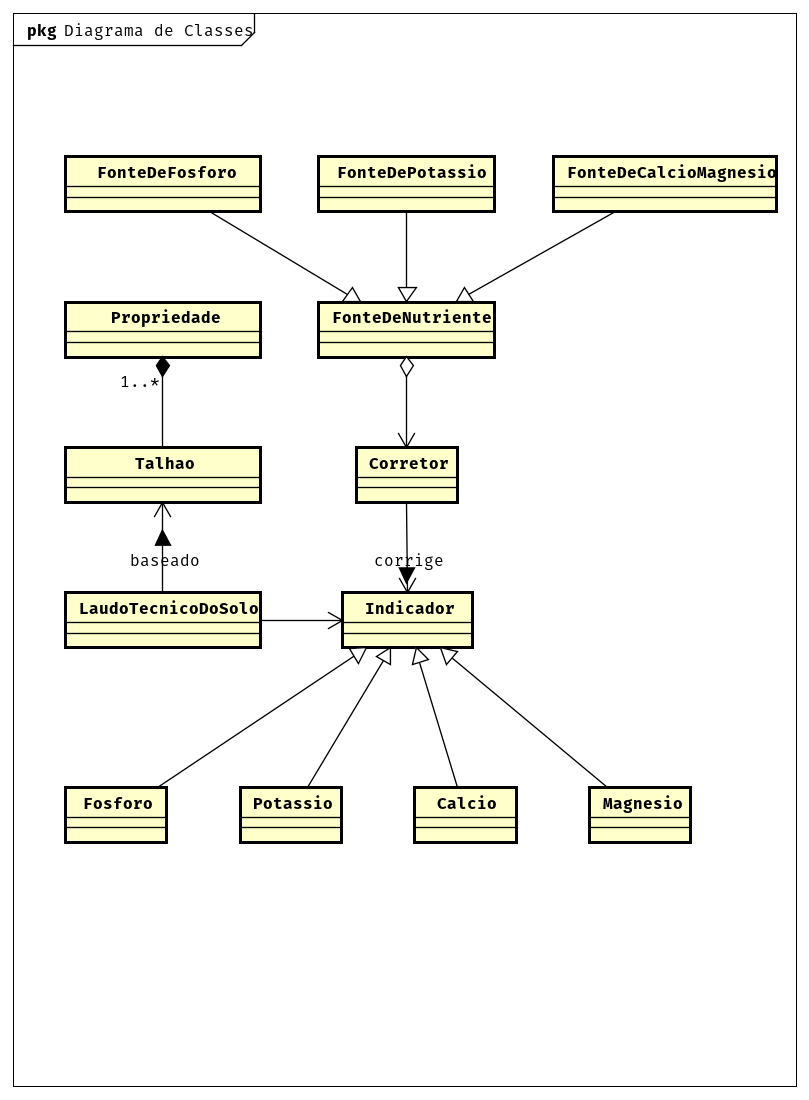
\includegraphics[width=13cm]{./dados/analise/diagramaclasse.png}
    \label{fig:diagramaClasse}
    \fonte{Autoria própria}
\end{figure}